\documentclass[a1,portrait]{a0poster}
\usepackage[absolute]{textpos}
\usepackage{graphicx}
\usepackage{times}
\usepackage{amsfonts}

%\usepackage[applemac]{inputenc}
\usepackage[T1]{fontenc}
%\usepackage{kmath,kerkis}
\usepackage{microtype}
\usepackage{tikz}
\parskip1ex plus.7ex minus.3ex %spazia di una riga 
\parindent0pt
\usepackage{amssymb, pb-diagram}
\usepackage{amsmath}
\usepackage{amsthm}
\usepackage{mathrsfs}
\usepackage{amsopn}
\usepackage[all]{xy}
\usepackage{color}
%\definecolor{red}{rgb}{0.8,0.0,0.1}
%\definecolor{blue}{rgb}{0.01,0.02,0.49}
%\definecolor{lightgray}{rgb}{0.45,0.50,0.65}
% see documentation for a0poster class for the size options here

\let\Textsize\normalsize
\def\Head#1{{\noindent\raggedright{\large\textsf{\textbf{#1}}}\par}}
\def\SHead#1{\noindent{\normalsize \textsf{#1}}}
\def\Title#1{\noindent{\Huge\color{red} \textsf{#1}}}
\def\Subtitleline#1{\noindent{\large \textsf{#1}}}

\newcommand{\alert}[1]{{ \textbf{#1}}}

\newtheorem{thm}{Theorem}
% Grid setup:

\TPGrid[25mm,25mm]{17}{25}  % 5 - 1 - 5 - 1 - 5 Columns

% Other settings

\pagestyle{empty}
\setcounter{secnumdepth}{0}

\parindent=0pt
\parskip=0.5\baselineskip

\renewcommand\refname{\SHead{References}\par\vspace*{-1ex}}


\begin{document}


%\TPshowboxestrue

% Poster title: -----------------------------------------------------




\begin{minipage}[c][9cm][c]{\textwidth}
  \begin{center}
    {\sc \Huge How is the Web like a snowflake?}\\[10mm]
    {\large D.Matthews \texttt{ dm1x07@soton.ac.uk}\\[7.5mm]
     \large Supervisors: Dr. J. Anderson, Dr. R. Carare\\[7.5mm]}  
     \includegraphics[scale=0.2]{./soton.jpeg}   
     \end{center}
\end{minipage}


\begin{textblock}{17.4}(-.2,3.1)
\rule{17.4\TPHorizModule}{1.8mm}
\end{textblock}

\sloppy


% First text block on the left: -------------------------------------

\begin{textblock}{8}(0,3.9)

\Head{Fractals} 
In the late 1600s Leibnitz studied structures that appear the same when we view them (or an appropriate substructure) at different length scales.  An example from nature of such a structure is the fern which we would find it difficult to distinguish from a magnified fern leaf or an extremely magnified fern leaf's smaller leaf. Surprisingly it was not until the 1960s and arguably the development of computers that Benoit Mandelbrot coined the word "fractal" for these types of object and thrust fractals firmly into the public imagination.  In mathematics models of random processes and geometry are fertile sources of fractals, Figure 1 below shows the Mandelbrot set which is a fractal arising from pure mathematics. Two reason that fractals became popular in the academic and wider world are:
\begin{itemize}
\item[(i)] They occur naturally, for example fern leaves and snowflakes are very nearly fractals.  
\item[(ii)] They are beautiful and have inspired artists such as Jackson Pollock.
\end{itemize}

\begin{figure}
\centering
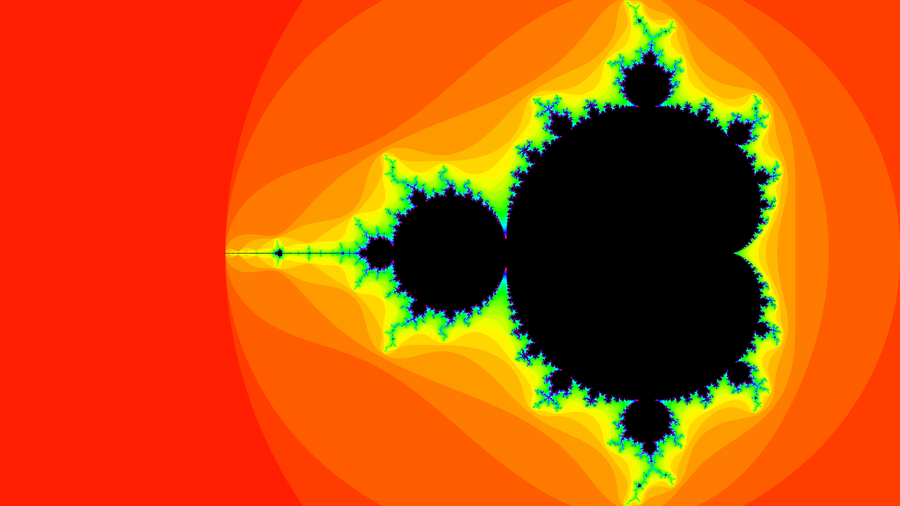
\includegraphics[scale=0.75]{frac.png}
\caption{The Mandelbrot set}
\label{fig:joetwat}
\end{figure}



\Head{Graphs}
Fractal structures also appear naturally in the study of random graphs.  Loosely speaking a graph $G$ consists of a set of nodes $N$ and a set of edges $E$ together with a function that assigns the two ends of each edge to a node.  We write $G = G(N,E)$.

As well as being interesting of themselves graphs have  successfully  been used to represent  a variety of real-world phenomena.  For example we can represent the Web as a graph by assigning every webpage to a node and then linking two nodes if the associated webpages are linked.  This model is so well established it has been named the Web graph. One way of modelling the Web, particularly the growth of the Web is by building a graph using a random process which adds nodes and edges over time.  

Representing phenomena like the Web by a graph is useful because properties of the graph such as the degree of each vertex (how many edges subtend a node) represent real world data such as the number of links that a webpage has.  Given a graph $G$, we can construct a new graph by taking any subset, $M$, of $N$ and all edges in $E$ that have both ends assigned to a node in $M$.  We calls such a graph a subgraph of $G$.  A simplified social network site consisting of a set of webpages associated to people and links between them corresponding to social interaction can be thought of as a subgraph of the Web graph.

A graph in which every two nodes are joined by following a \emph{unique} series of edges from end to end is called a \emph{tree}.  Trees are easier to calculate with and the following theorem marries graphs with trees.

\begin{thm}
Every graph $G = G(N_{1},E_{1})$ admits a spanning subgraph $T = T(N_{2},E_{2})$ such that $T$ is a tree.  
\end{thm}
By a spanning tree we mean a tree $T$ such that $N_{1} = N_{2}$.

Further, ....argue that spanning trees of the Web graph can be thought of as an information kernel of information motorways for the more complicated network they span. 



\end{textblock}

% Right text block: ------------------------------------------------ 
\begin{textblock}{8}[1,0](17,3.9)



\Head{Properties of Graphs}
We have seen that graphs or networks are built from nodes and edges and can be associated with a vast array of natural, social and technical phenomena.  Remarkably this array includes examples as diverse as the Web, the cerebral arterial tree and the metabolism of \emph{E. Coli}.  What is even more astonishing is that all these networks, along with countless others exhibit the following two properties:

\begin{itemize}
\item[(i)] \emph{ the small-world property} Given a pair of nodes in the network there exists a path along edges and nodes which is incredibly short relative to the size of the network as a whole.
\item[(ii)] \emph{scale free behaviour}  If we plot the degree of a node against the number of nodes with that degree we get a decreasing power law.
\end{itemize}

We should note that scale free does not necessarily mean that we can consider these networks fractal but there is a close correspondence.  

\Head{Current research}

In order to answer the question, "to what extent are these networks fractal?" we have conducted a survey of biological and technical, graphs and particularly trees with the aim of generating multidisciplinary questions pertaining to the structure of the Web graph and its various subgraphs.  In particular we focused our attention on Altzheimer's disease since geometric features such as the average degree of the cerebral arterial tree plays a pivotal role in the progression of this disease.  By designing and investigating models of Altzheimer's disease we are able to draw parallels between the 'natural' structure of the cerebral vasculature and the structure of an online social network. 

Murray's law of  least work\cite{} states that a natural process will evolve to minimize its energy loss as is possible drive the geometric structure of the cerebral vasculature.  This naturally begs the questions: what is the extent to which online social networks exhibit fractal properties and are there technological and social equivalents of Murray's law? 

\begin{figure}
\centering
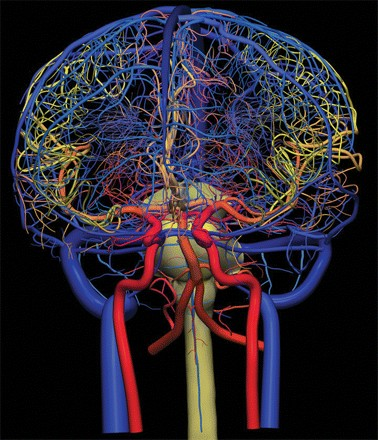
\includegraphics[scale=0.3]{veins.jpg}
\caption{An computer generated image of the cerebral vascular tree}
\label{fig:joetwat}
\end{figure}


\Head{Future work}
Confusion about the precise definition of fractal pervades the literature describing biological and technical networks and words such as 'self-similar are used without due regard for the mathematical definition.  Essential further work includes making these previous works more rigorous. 
\begin{figure}
\centering
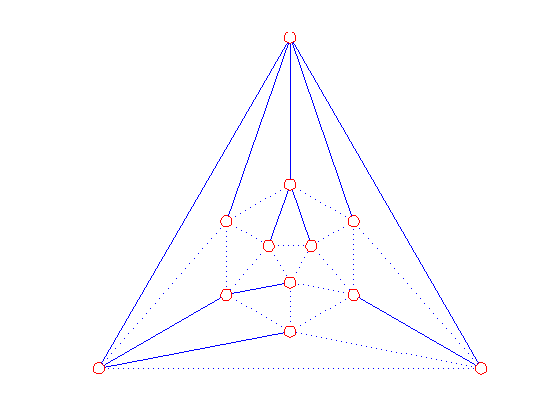
\includegraphics[scale=0.52]{spa.png}
\caption{A graph in which the spanning tree has been highlighted in blue}
\label{fig:joe2}
\end{figure}

\end{textblock}

% References: -------------------------------------------------------

\begin{textblock}{8}[1,1](17,25.4)
    \small 
    

%\bibliography{/home/jtait/Desktop/Work/Bibliography/biblio.bib}
%\bibliographystyle{plain}
\begin{thebibliography}{9}
\bibitem{Goh}
K.I. Goh, B. Salvi, B. Kahng, and D. Kim. "Skeleton and Fractal Scaling in Complex Networks". \emph{Physical Review Letter}, 96, 018701, 2006.
\bibitem{Murray}
C.D. Murray. "The Physiological Principle of
Minimum Work: I. The Vascular System
and the Cost of Blood Volume". \emph{Proc. Natl.
Acad. Sci. U.S.A.}, 12(3):207-214, 1926.
\bibitem{Su}
S-W. Su, M. Catherall and S. Payne. "The Influence of Network Structure on the Transport of Blood in the Human Cerebral Microvasculature". \emph{Microcirculation}, 19:175-187, 2012.
\end{thebibliography}
\end{textblock}






% --------------------------------------------------------------------

\end{document}

